\subsection{Design System}
\label{sec:design-system}

% Ô màu cho bảng token
\newcommand{\sw}[2]{\colorbox[HTML]{#1}{\textcolor[HTML]{#2}{\rule{0pt}{0.35cm}\hspace{0.7cm}}}}

Design system của OneSpace được xây trên \textbf{Material 3}~\cite{material3} và tổ chức hoàn toàn theo \textit{token theo vai trò} (role-based): mã nguồn không-hardcode màu, mọi màn hình đều tham chiếu các vai trò màu của Material Theme (\texttt{primary}, \texttt{onSurface}, \texttt{surfaceContainer}, \ldots) được định nghĩa tập trung trong một tệp theme duy nhất của ứng dụng. Cách đặt tên theo vai trò này bảo đảm khi thay đổi bảng màu, toàn bộ giao diện cập nhật đồng loạt mà không cần sửa từng màn hình~--~đây cũng là câu trả lời cho câu hỏi tái sử dụng token khi lập trình: một token được khai báo một lần, dùng ở mọi nơi.

Bảng màu theo định hướng thương hiệu \textit{mint--teal trên nền xanh mực}: màu chính light là xanh lá đậm (đậm hơn nền một bậc), ở dark chuyển thành mint sáng; màu phụ là teal. Mọi vai trò đều được khai báo thành cặp \texttt{role/onRole} (chữ trên nền tương ứng) để component tự giữ tương phản đọc được ở cả hai chế độ. Bảng~\ref{tab:design-tokens} liệt kê các token tiêu biểu; giá trị hex lấy trực tiếp từ mã nguồn theme của ứng dụng.

\begin{table}[H]
\centering
\small
\caption{Design token màu theo vai trò Material 3}
\label{tab:design-tokens}
\begin{tabularx}{\textwidth}{@{}>{\raggedright\arraybackslash}p{3.5cm} >{\centering\arraybackslash}p{1.3cm} >{\raggedright\arraybackslash}X@{}}
\toprule
\textbf{Vai trò (Light / Dark)} & \textbf{Màu} & \textbf{Dùng cho} \\
\midrule
primary / onPrimary \newline 41690F / B8F36E & \sw{41690F}{B8F36E} & Nút chính, tab đang chọn, liên kết \\
primaryContainer \newline C3F491 / 334E00 & \sw{C3F491}{334E00} & Vùng nhấn mạnh, nền icon thẻ \\
secondary / onSecondary \newline 006A68 / 9BD8D1 & \sw{006A68}{9BD8D1} & Nút phụ, chip chuyên mục \\
tertiary / onTertiary \newline 566516 / BDE886 & \sw{566516}{BDE886} & Điểm nhấn phụ (gamification) \\
error / onError \newline BA1A1A / FFB4AB & \sw{BA1A1A}{FFB4AB} & Thông báo lỗi, nút thử lại \\
background / onBackground \newline F8FAF2 / 10140E & \sw{F8FAF2}{10140E} & Nền màn hình và chữ chính \\
surface / onSurface \newline F8FAF2 / 10140E & \sw{F8FAF2}{10140E} & Bề mặt card, thanh công cụ \\
surfaceVariant \newline DEE3D0 / 43483D & \sw{DEE3D0}{43483D} & Chữ phụ, nền chip \\
surfaceContainer\allowbreak{}High \newline E5E8D6 / 272F25 & \sw{E5E8D6}{272F25} & Card nổi, dock mini player \\
outline \newline 75796D / 8E927F & \sw{75796D}{8E927F} & Viền phân tách, gợi ý ô nhập \\
\bottomrule
\end{tabularx}
\end{table}

Hai quyết định quan trọng về màu:

\begin{itemize}
    \item \textbf{Chế độ tối đi theo hệ thống, có ghi đè thủ công.} Ứng dụng đọc chế độ tối của hệ điều hành làm mặc định (tương ứng F-COM-13); trong Cài đặt người dùng chọn được Sáng, Tối hoặc Theo hệ thống~--~tùy chọn này được lưu và áp dụng cho toàn bộ ứng dụng ở lần mở sau.
    \item \textbf{Dynamic color tắt mặc định.} Android 12+ cho phép lấy màu theo hình nền của người dùng (dynamic color); ứng dụng hỗ trợ cơ chế này nhưng tắt mặc định để nhận diện thương hiệu mint--teal ổn định trên mọi thiết bị, vì bảng màu là một phần nhận diện sản phẩm chứ không phải trang trí.
\end{itemize}

Hình~\ref{fig:design-modes} so sánh cùng ba màn hình ở hai chế độ: cùng một hệ vai trò token giữ bố cục nguyên vẹn, chỉ đổi giá trị màu.

\begin{figure}[H]
\centering
\begin{minipage}{0.31\textwidth}\centering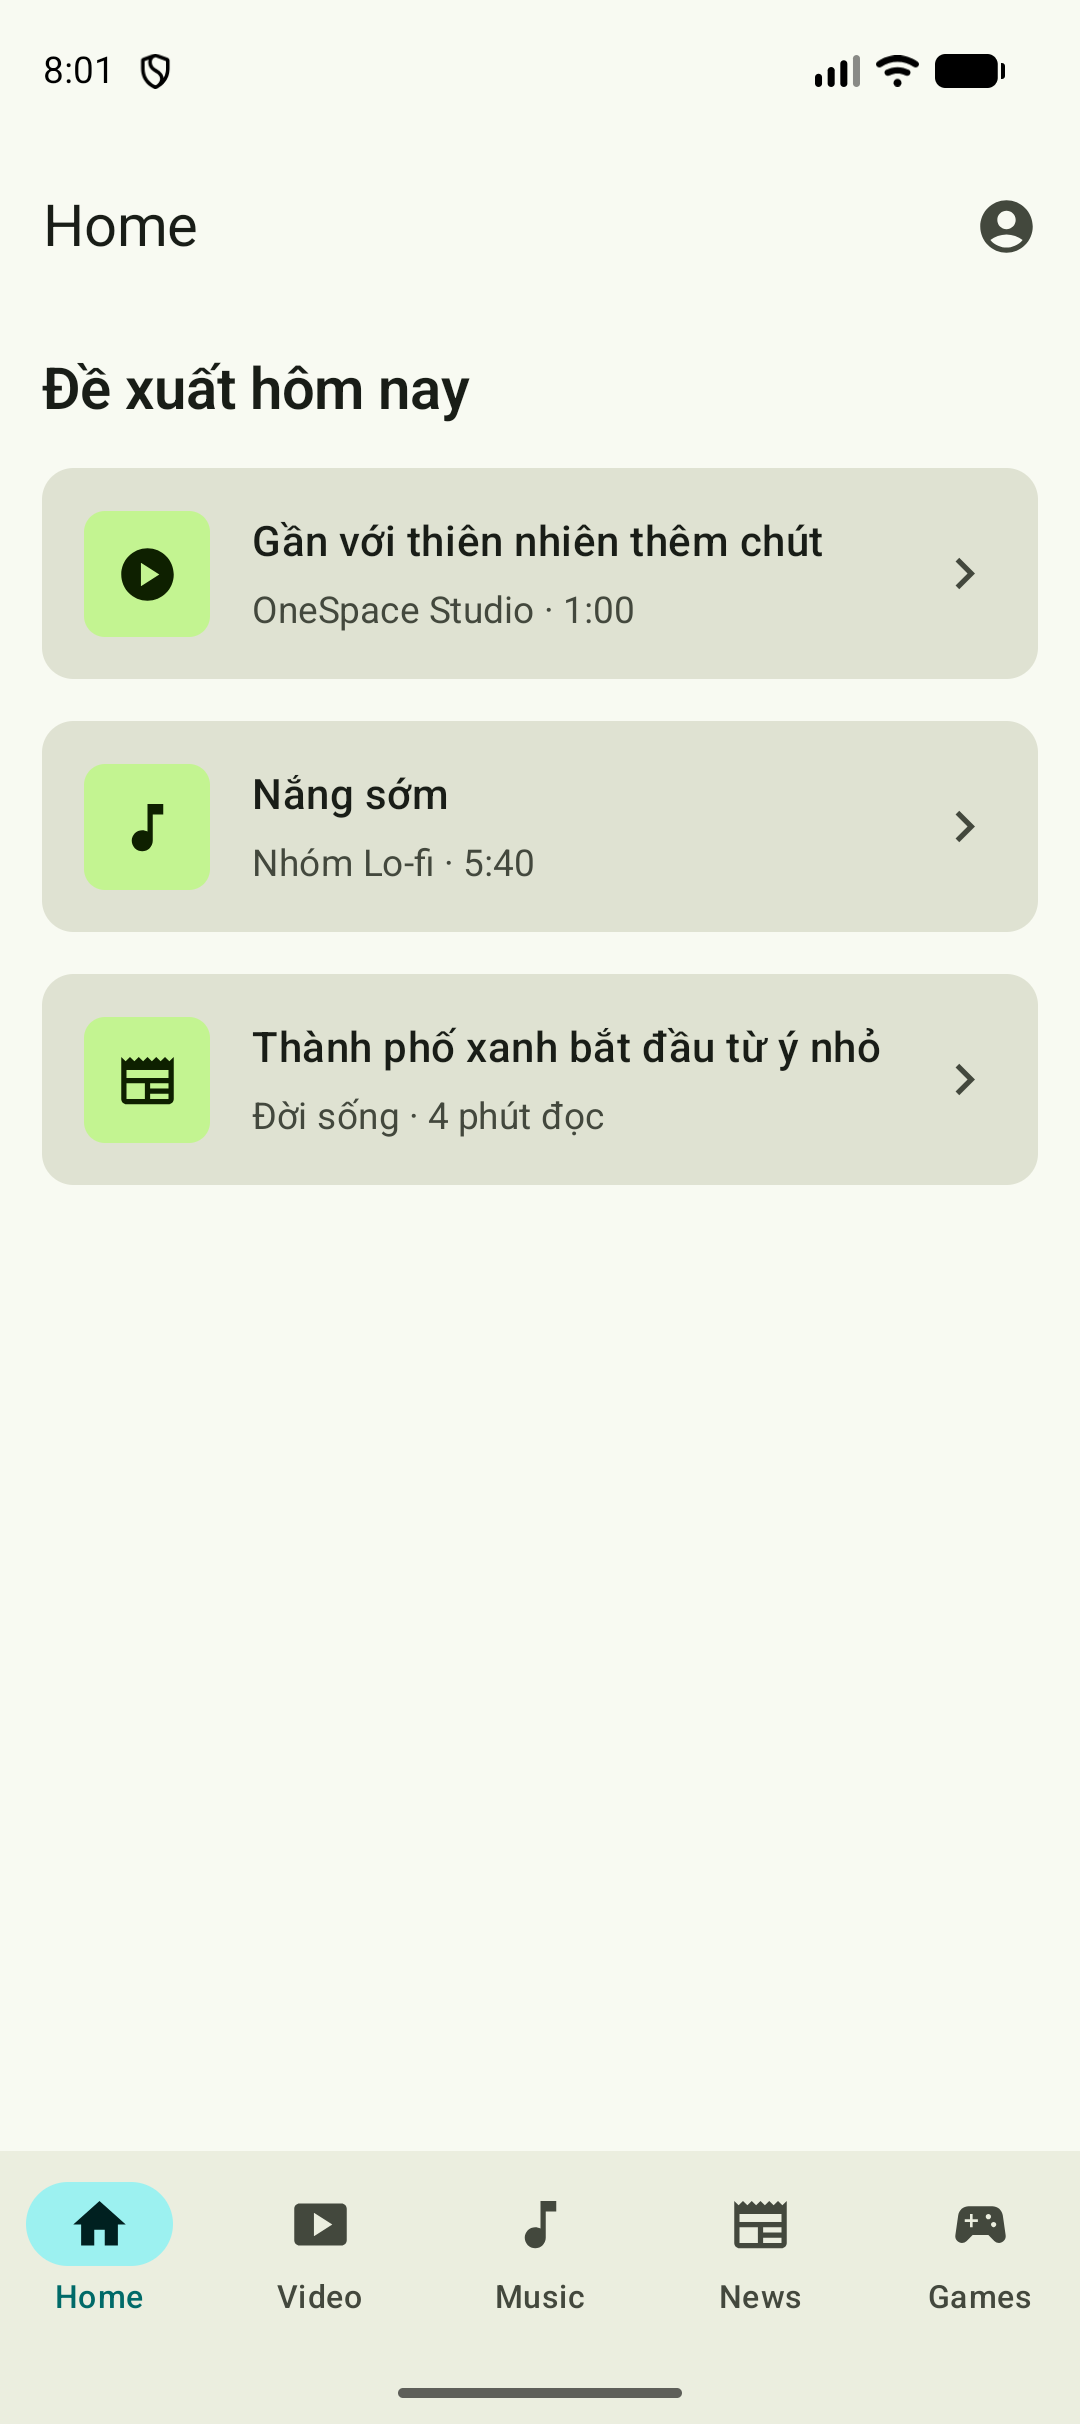
\includegraphics[width=0.86\textwidth]{figures/app/home-light.png}\end{minipage}\hfill
\begin{minipage}{0.31\textwidth}\centering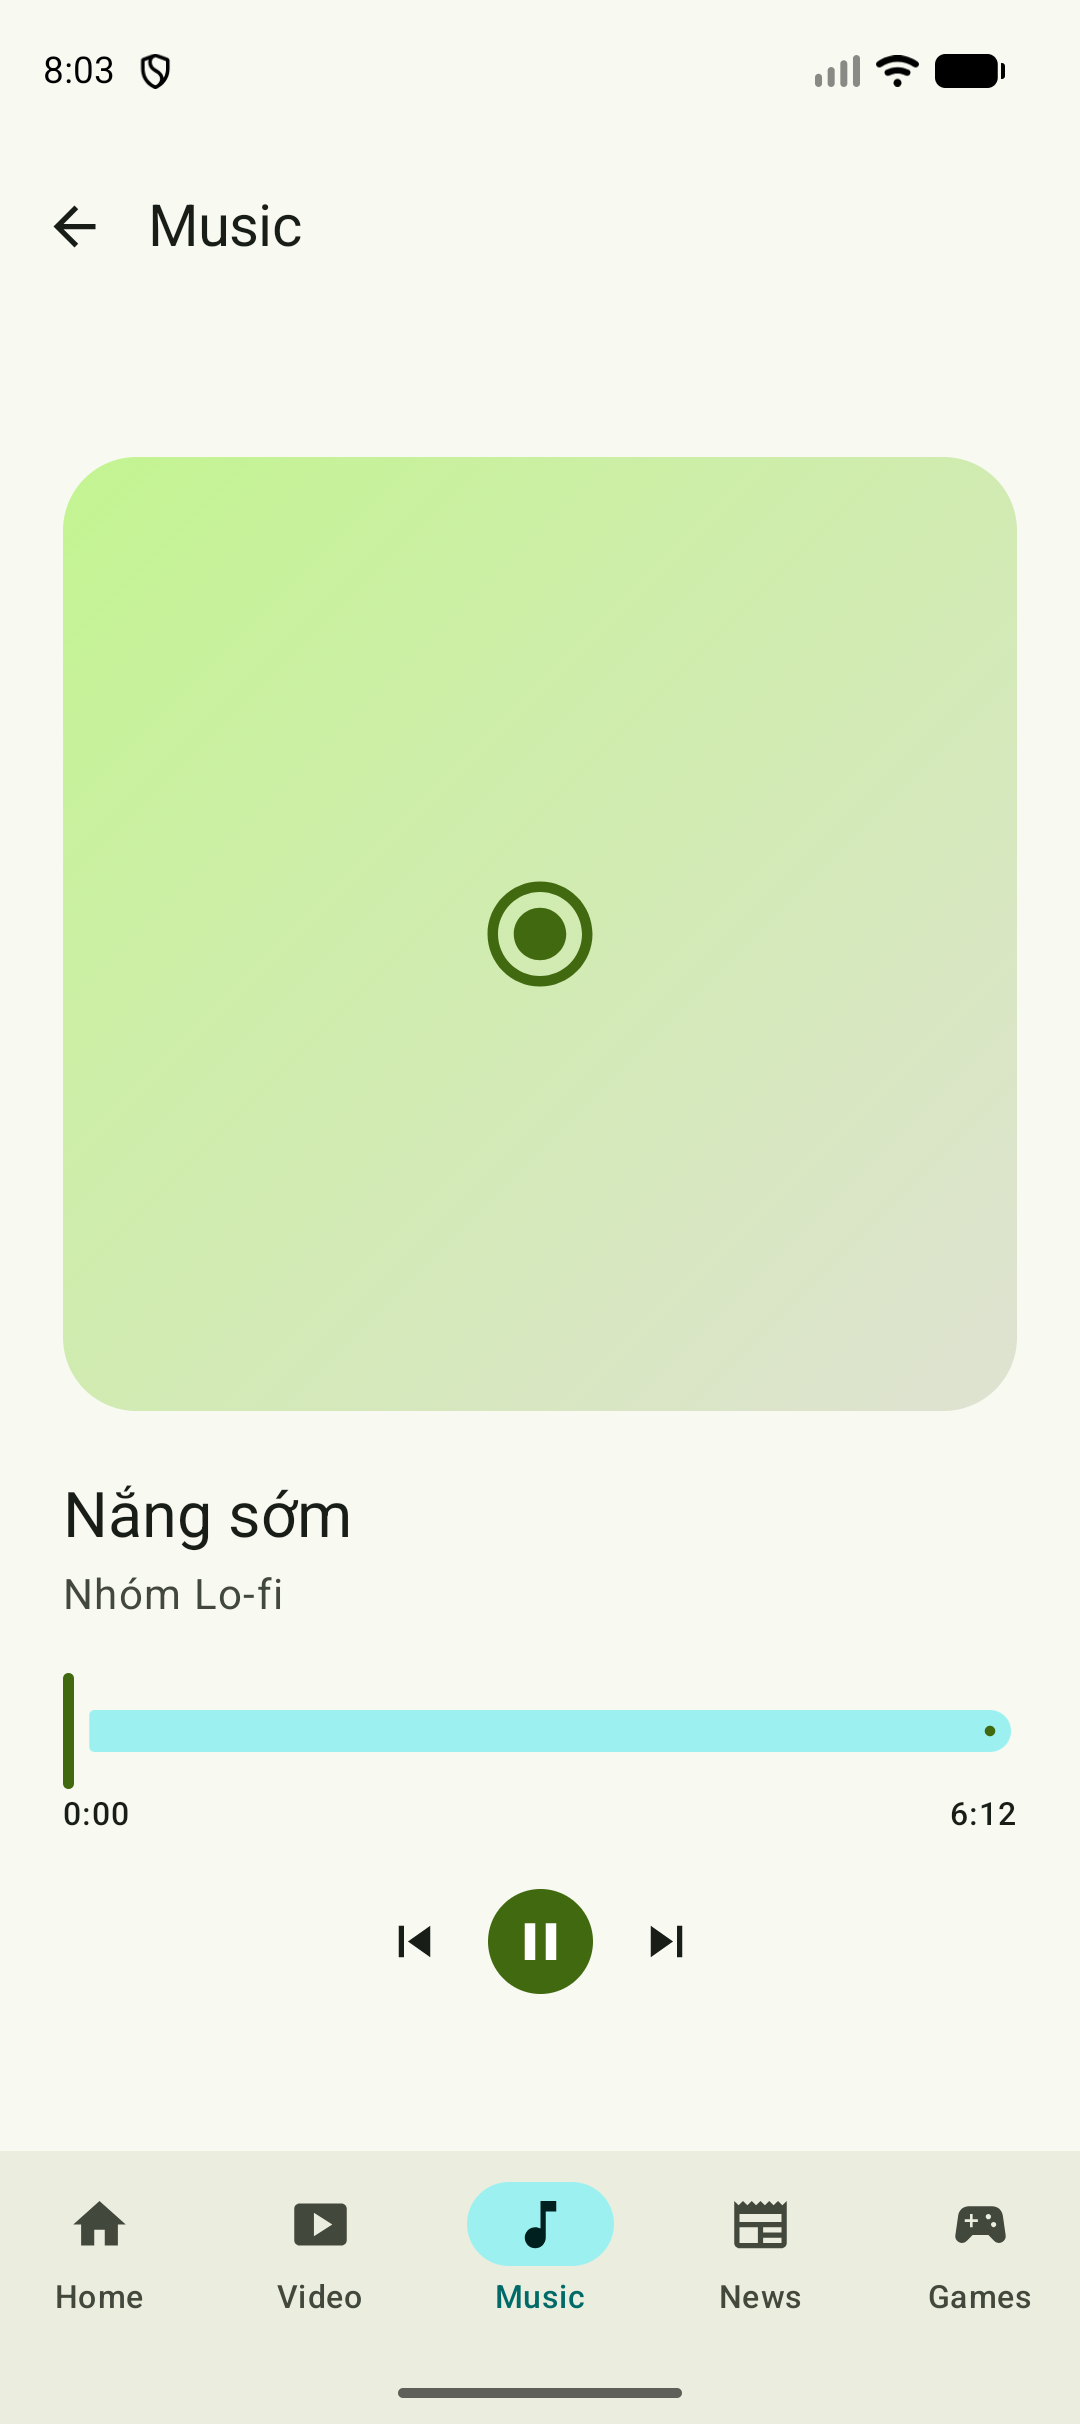
\includegraphics[width=0.86\textwidth]{figures/app/now-playing-light.png}\end{minipage}\hfill
\begin{minipage}{0.31\textwidth}\centering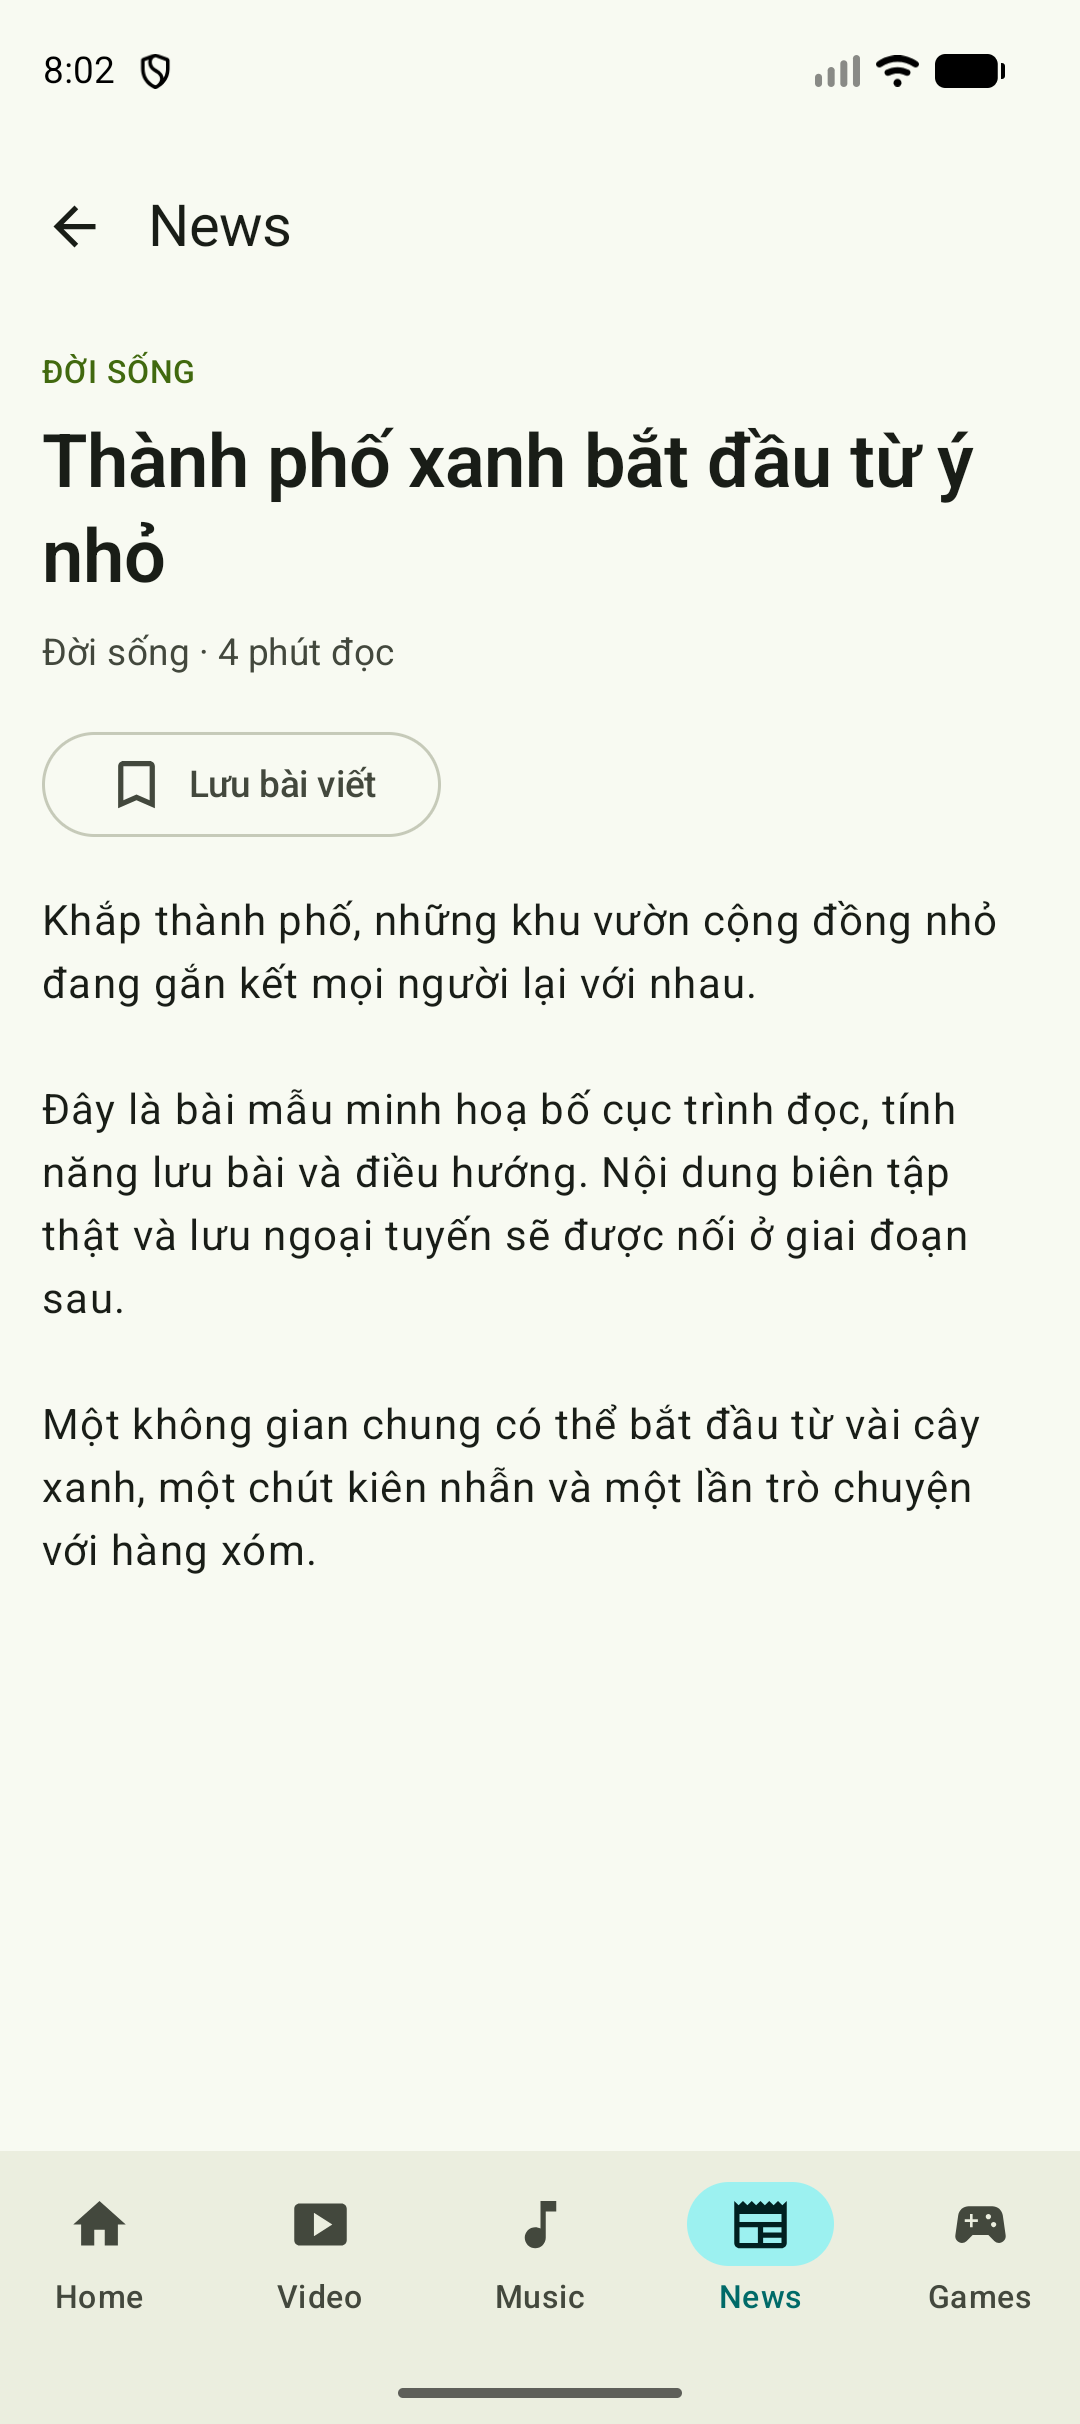
\includegraphics[width=0.86\textwidth]{figures/app/article-light.png}\end{minipage}

\vspace{4pt}

\begin{minipage}{0.31\textwidth}\centering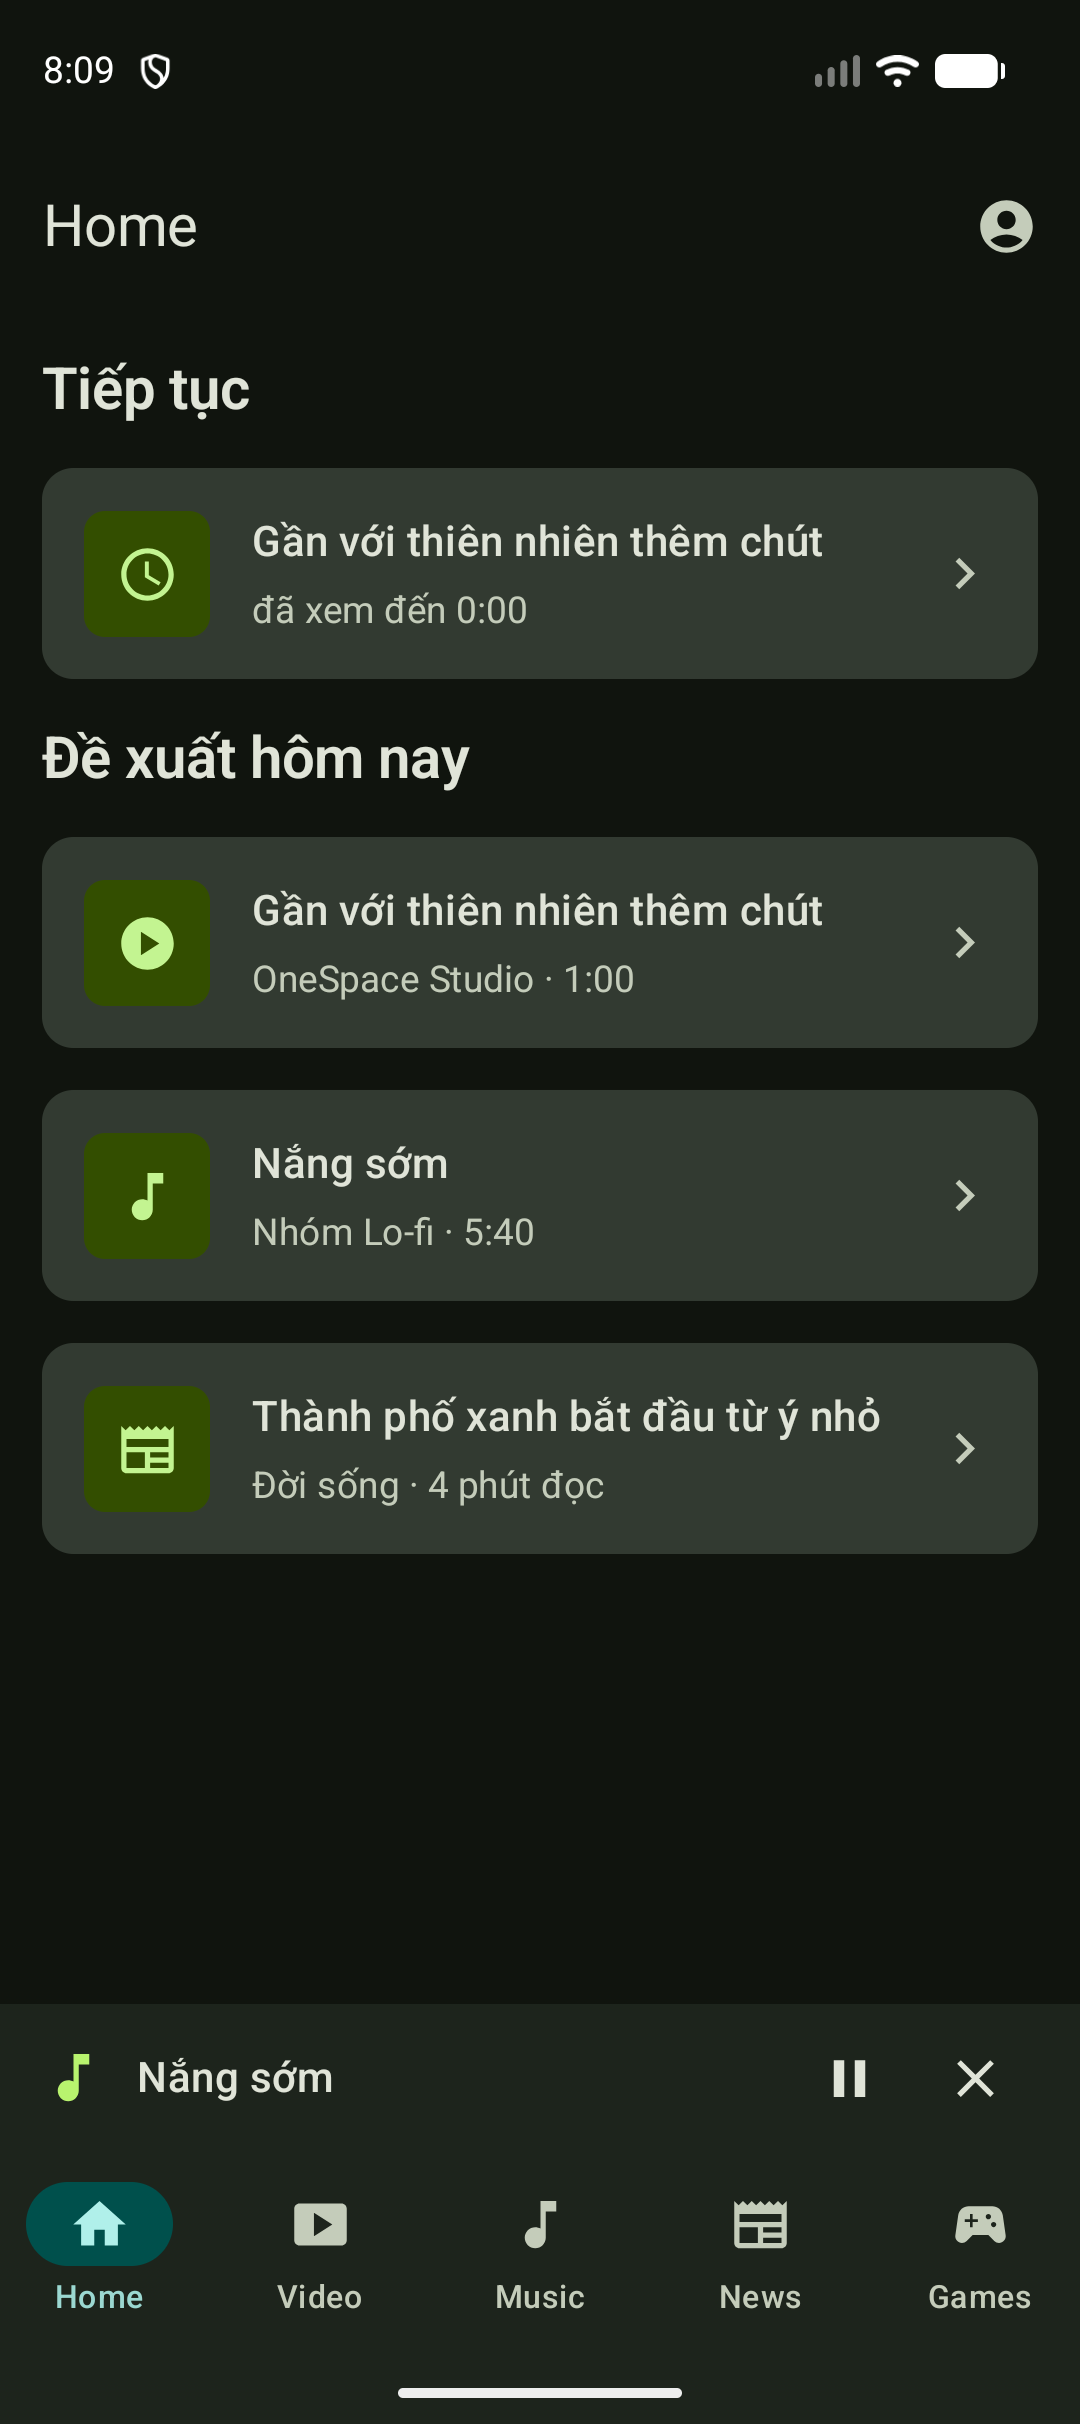
\includegraphics[width=0.86\textwidth]{figures/app/home-dark.png}\end{minipage}\hfill
\begin{minipage}{0.31\textwidth}\centering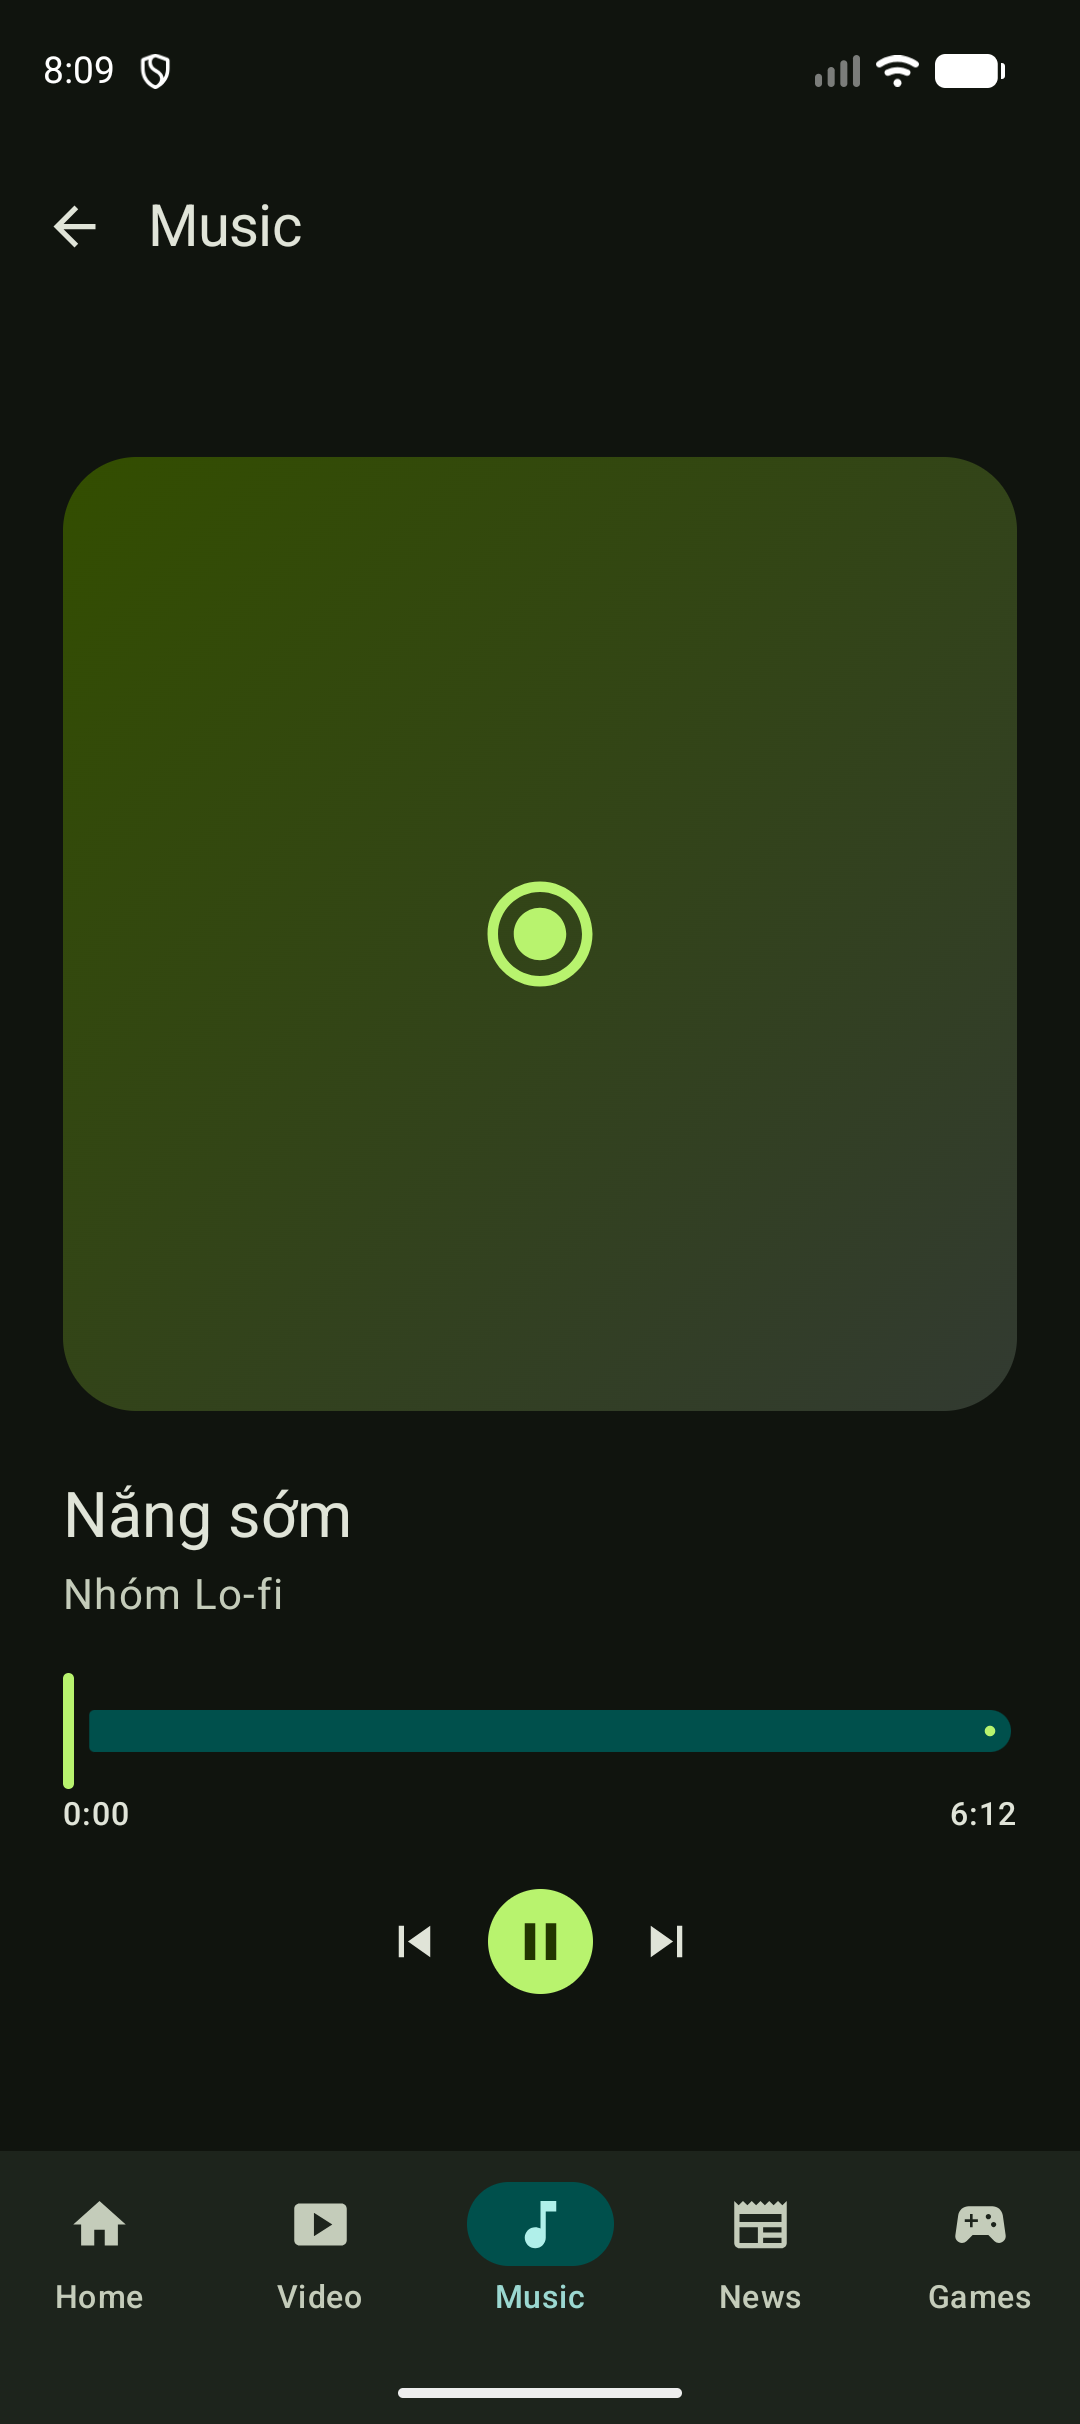
\includegraphics[width=0.86\textwidth]{figures/app/now-playing-dark.png}\end{minipage}\hfill
\begin{minipage}{0.31\textwidth}\centering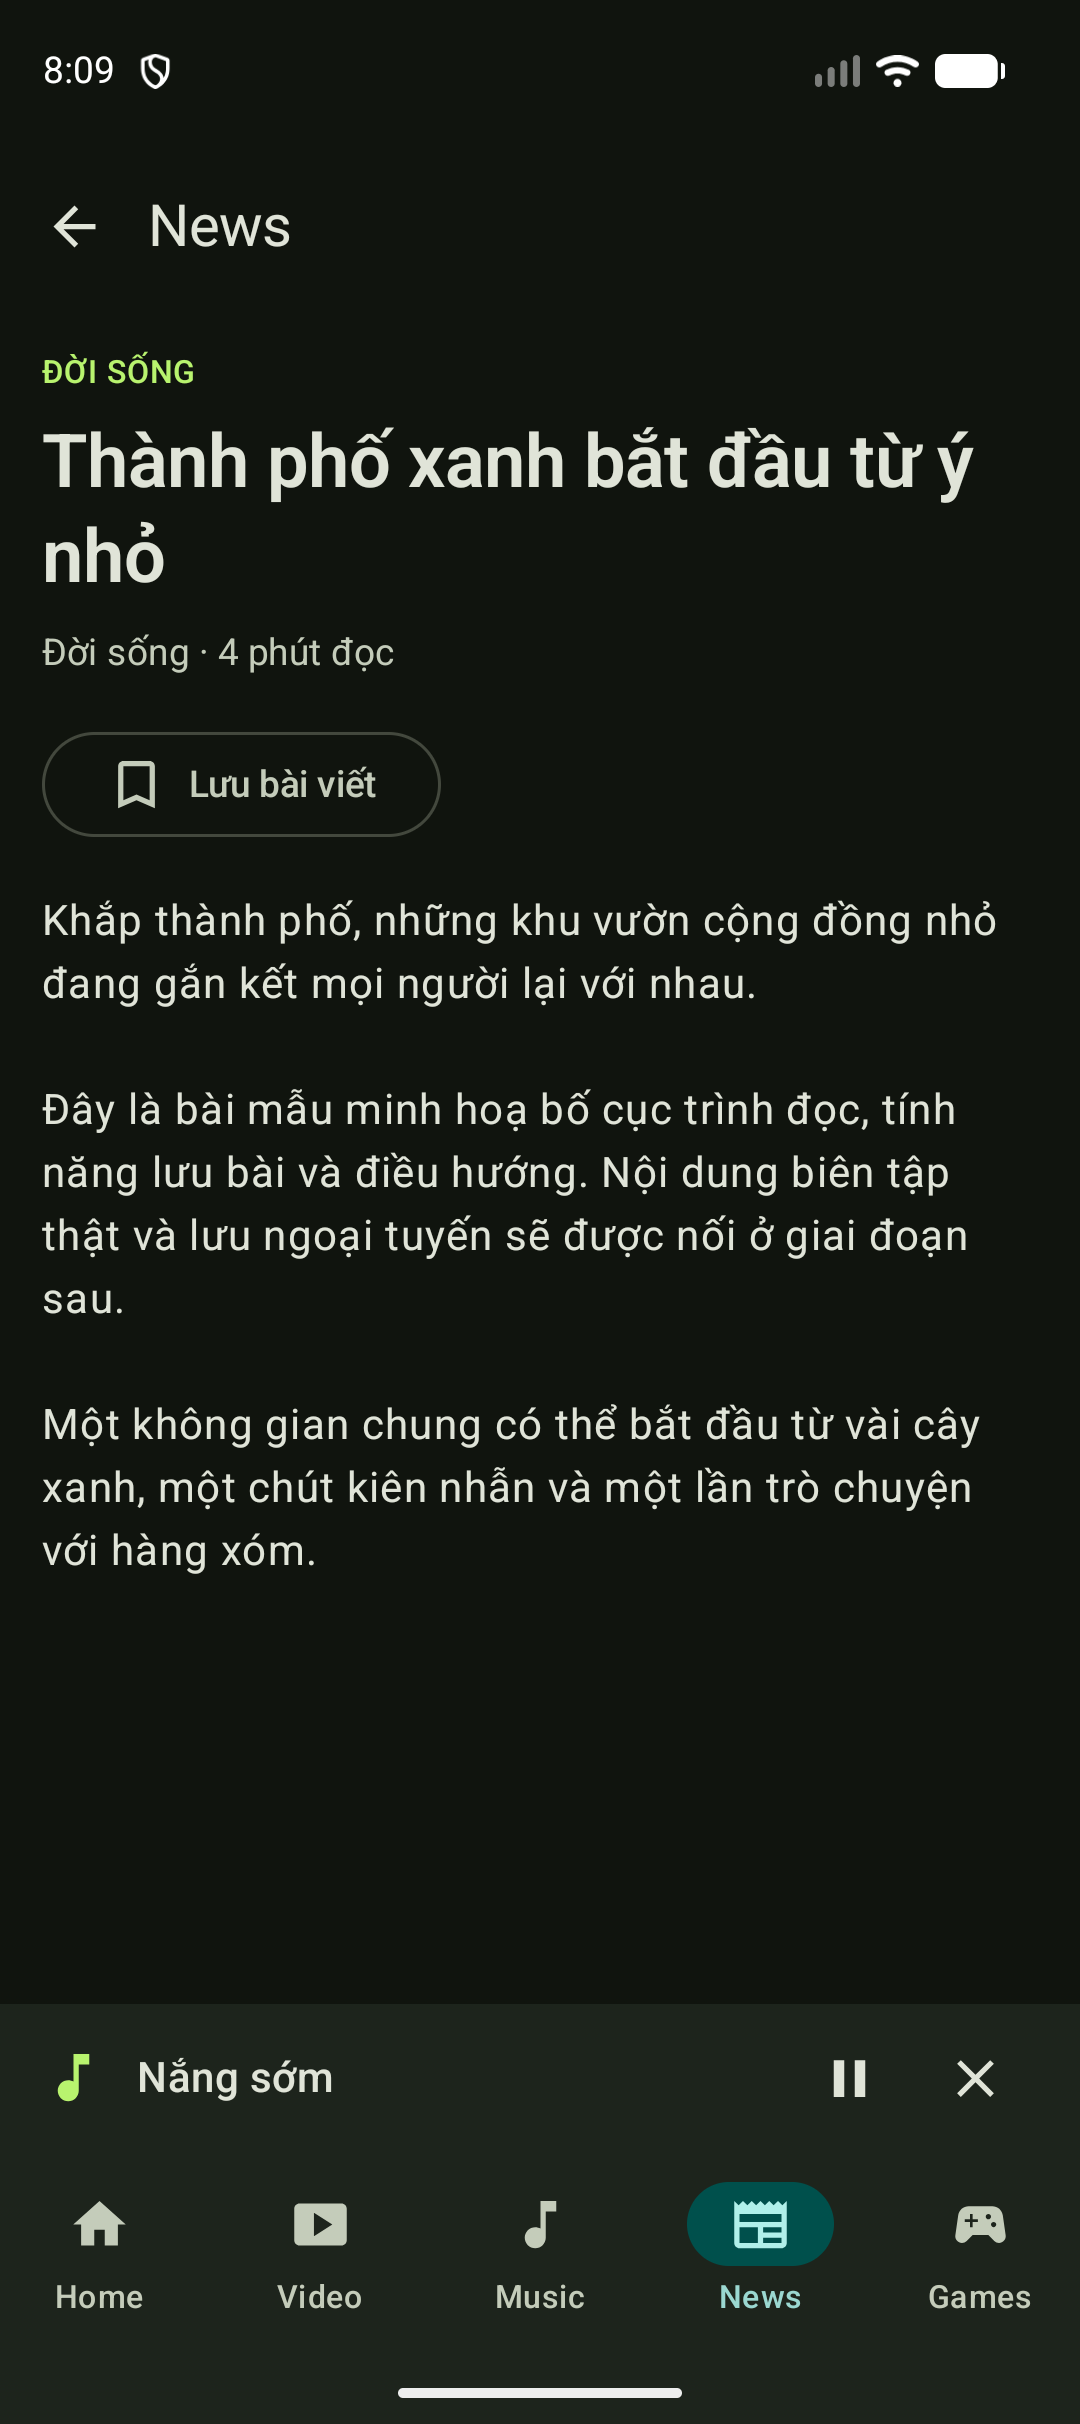
\includegraphics[width=0.86\textwidth]{figures/app/article-dark.png}\end{minipage}
\caption{Cùng ba màn hình ở chế độ sáng (trên) và tối (dưới): token giữ nguyên vai trò, chỉ đổi giá trị}
\label{fig:design-modes}
\end{figure}

\textbf{Typography.} Ứng dụng dùng nguyên thang chữ mặc định của Material 3 (display, headline, title, body, label) mà không định nghĩa kiểu chữ riêng. Quyết định này có chủ đích: thang M3 đã được hiệu chỉnh theo chuẩn đọc của Android, và mọi cỡ chữ đều đặt theo đơn vị \texttt{sp} nên tự phóng to theo cài đặt cỡ chữ hệ thống (chi tiết ở mục~\ref{sec:accessibility}). Việc thay font thương hiệu riêng, nếu có, sẽ là một thay đổi token tập trung duy nhất ở tệp theme.

\textbf{Component library.} Bảng~\ref{tab:component-library} phân loại component của ứng dụng: lớp \textit{dùng chung} định nghĩa trong module design system và được cả bốn phân hệ tham chiếu (đây là phần ``thư viện'' thật sự của design system); lớp \textit{theo chuẩn Material 3} dùng trực tiếp component nền tảng; các màn đặc thù tự dựng từ hai lớp này.

\begin{table}[H]
\centering
\caption{Thư viện component của OneSpace}
\label{tab:component-library}
\begin{tabularx}{\textwidth}{>{\raggedright\arraybackslash}p{3.4cm} >{\raggedright\arraybackslash}X}
\toprule
\textbf{Component} & \textbf{Vai trò} \\
\midrule
\multicolumn{2}{l}{\textit{Dùng chung (module design system)}} \\
\texttt{FeaturePage} & Khung trang cho mọi feed: padding ngang 16dp, khoảng cách dọc 16dp giữa các phần. \\
\texttt{SectionTitle} & Nhãn tiêu đề phần trong feed (``Tiếp tục'', ``Đề xuất hôm nay'', ``Liên quan''). \\
\texttt{ContentCard} & Thẻ nội dung dùng chung cho cả bốn phân hệ: biểu tượng trong vùng primaryContainer, tiêu đề, phụ đề và nút mở. \\
\texttt{CatalogContent} & Bộ chuyển trạng thái của mọi feed: đang tải $\rightarrow$ skeleton, lỗi/offline $\rightarrow$ thông điệp + thử lại, rỗng $\rightarrow$ thông điệp + nút hành động, có dữ liệu $\rightarrow$ nội dung. \\
\texttt{SkeletonFeed} & Bốn hàng khung xám chạy hiệu ứng shimmer thay cho feed đang tải. \\
\texttt{EmptyState} / \texttt{ErrorState} & Trạng thái rỗng (kèm nút hành động) và trạng thái lỗi (kèm ``Thử lại''). \\
\midrule
\multicolumn{2}{l}{\textit{Theo chuẩn Material 3}} \\
Bottom Navigation, ListItem, Switch, Button / OutlinedButton, Modal Bottom Sheet & Thanh 5 tab, hàng cài đặt, công tắc, nút, sheet xác nhận chế độ dùng thử. \\
\midrule
\multicolumn{2}{l}{\textit{Đặc thù từng phân hệ}} \\
Trình phát video + cửa sổ nổi, Now Playing, trình đọc bài, bàn chơi 2048 & Tự dựng theo bố cục riêng, vẫn dùng token và component chung ở trên. \\
\bottomrule
\end{tabularx}
\end{table}

Về quy chuẩn nền tảng: ứng dụng Android-native tuân theo Material Design~\cite{material3} cho toàn bộ ngôn ngữ tương tác~--~ripple khi chạm, elevation của card và bottom sheet, vùng chạm tối thiểu 48dp, motion theo chuẩn M3. Nhóm không áp dụng song song Apple Human Interface Guidelines vì sản phẩm chỉ phát hành trên Android (quyết định chọn nền tảng ở Phần~\ref{sec:technical-architecture}); giữ một quy chuẩn nền tảng duy nhất cũng giúp giao diện nhất quán hơn là pha trộn hai bộ quy chuẩn khác nhau.
